\documentclass[spanish,a4paper]{article}

% Paquetes generales
\usepackage{ifthen}
\usepackage{amssymb}
\usepackage{amsmath}
\usepackage{multicol}
\usepackage[absolute]{textpos}
\usepackage{hyperref}
%\usepackage{graphicx}
\usepackage{caratula}

\setlength{\parindent}{12pt}

%% **************************************************************************
%
%  Package 'caratula', version 0.3 (para componer caratulas de TPs del DC).
%
%  CON MINIMAS MODIFICACIONES DEL TEAM ORGA2
%
%  En caso de dudas, problemas o sugerencias sobre este package escribir a
%  Brian J. Cardiff (bcardif arroba gmail.com).
%  Nico Rosner (nrosner arroba dc.uba.ar).
%
% **************************************************************************

% ----- Informacion sobre el package para el sistema -----------------------

\NeedsTeXFormat{LaTeX2e}
\ProvidesPackage{caratula}[2005/08/09 v0.3 Para componer caratulas de TPs del DC]
%\usepackage[pdftex]{graphicx}

% ----- Imprimir un mensajito al procesar un .tex que use este package -----

\typeout{Cargando package 'caratula' v0.3 (2005/08/09)}

% ----- Algunas variables --------------------------------------------------

\let\Materia\relax
\let\Submateria\relax
\let\Titulo\relax
\let\Subtitulo\relax
\let\Grupo\relax
\let\Fecha\relax
\let\Logoimagefile\relax

% ----- Comandos para que el usuario defina las variables ------------------

\def\materia#1{\def\Materia{#1}}
\def\submateria#1{\def\Submateria{#1}}
\def\titulo#1{\def\Titulo{#1}}
\def\subtitulo#1{\def\Subtitulo{#1}}
\def\grupo#1{\def\Grupo{#1}}
\def\fecha#1{\def\Fecha{#1}}
\def\logoimagefile#1{\def\Logoimagefile{#1}}

% ----- Token list para los integrantes ------------------------------------

\newtoks\intlist\intlist={}

% ----- Comando para que el usuario agregue integrantes --------------------

\def\integrante#1#2#3{\intlist=\expandafter{\the\intlist
    \rule{0pt}{1.2em}#1&#2&\tt #3\\[0.2em]}}

% ----- Macro para generar la tabla de integrantes -------------------------

\def\tablaints{%
    \begin{tabular}[t]{| l @{\hspace{4ex}} c @{\hspace{4ex}} l|}
        \hline
        \multicolumn{1}{|c}{\rule{0pt}{1.2em} Integrante} & LU &  \multicolumn{1}{c|}{Correo electr\'onico} \\[0.2em]
        \hline \hline
        \the\intlist
        \hline
    \end{tabular}}

% ----- Codigo para manejo de errores --------------------------------------

\def\se{\let\ifsetuperror\iftrue}
\def\ifsetuperror{%
    \let\ifsetuperror\iffalse
    \ifx\Materia\relax\se\errhelp={Te olvidaste de proveer una \materia{}.}\fi
    \ifx\Titulo\relax\se\errhelp={Te olvidaste de proveer un \titulo{}.}\fi
    \edef\mlist{\the\intlist}\ifx\mlist\empty\se%
    \errhelp={Tenes que proveer al menos un \integrante{nombre}{lu}{email}.}\fi
    \expandafter\ifsetuperror}


% ----- \maketitletxt correspondiente a la versión v0.2 (texto) ---------

\def\maketitletxt{%
    \ifsetuperror\errmessage{Faltan datos de la caratula! Ingresar 'h' para mas informacion.}\fi
    \thispagestyle{empty}
    \begin{center}
    \vspace*{\stretch{2}}
    {\LARGE\textbf{\Materia}}\\[1em]
    \ifx\Submateria\relax\else{\Large \Submateria}\\[0.5em]\fi
    \par\vspace{\stretch{1}}
    {\large Departamento de Computaci\'on}\\[0.5em]
    {\large Facultad de Ciencias Exactas y Naturales}\\[0.5em]
    {\large Universidad de Buenos Aires}
    \par\vspace{\stretch{3}}
    {\Large \textbf{\Titulo}}\\[0.8em]
    {\Large \Subtitulo}
    \par\vspace{\stretch{3}}
    \ifx\Grupo\relax\else\textbf{\Grupo}\par\bigskip\fi
    \tablaints
    \end{center}
    \vspace*{\stretch{3}}
    \newpage}

% ----- \maketitle correspondiente a la versión v0.3 (gráfica) -------------

\def\maketitlegraf{%
    \ifsetuperror\errmessage{Faltan datos de la caratula! Ingresar 'h' para mas informacion.}\fi
%
    \thispagestyle{empty}

    \ifx\Logoimagefile\relax\else\includegraphics{\Logoimagefile}\fi\hfill 
\includegraphics{imagenes/logodc.jpg}

    \vspace*{.12 \textheight}

    \noindent \textbf{\huge \Titulo}  \medskip \\
    \ifx\Subtitulo\relax\else\noindent\textbf{\large \Subtitulo} \\ \fi%
    \noindent \rule{\textwidth}{1 pt}

    {\noindent\large\Fecha \hspace*\fill \Materia} \\
    \ifx\Submateria\relax\else{\noindent \hspace*\fill \Submateria}\fi%

    \medskip%
    \begin{center}
        \ifx\Grupo\relax\else\textbf{\Grupo}\par\bigskip\fi
        \tablaints
    \end{center}%
    \vfill%
%
    \begin{minipage}[t]{\textwidth}
        \begin{minipage}[t]{.55 \textwidth}
            
\includegraphics{imagenes/logouba.jpg}
        \end{minipage}%%
        \begin{minipage}[b]{.50 \textwidth}
            \textbf{\textsf{Facultad de Ciencias Exactas y Naturales}} \\
            \textsf{Universidad de Buenos Aires} \\
            {\scriptsize %
            Ciudad Universitaria - (Pabell\'on I/Planta Baja) \\
                Intendente G\"uiraldes 2160 - C1428EGA \\
            Ciudad Aut\'onoma de Buenos Aires - Rep. Argentina \\
                Tel/Fax: (54 11) 4576-3359 \\
            http://www.fcen.uba.ar \\
            }
        \end{minipage}
    \end{minipage}%
%
    \newpage}

% ----- Reemplazamos el comando \maketitle de LaTeX con el nuestro ---------

\def\maketitle{\maketitlegraf}

\begin{document}

\titulo{Trabajo Pr\'{a}ctico}
\subtitulo{}

\fecha{\today}

\materia{Organizaci\'{o}n Del Computador 2}
\grupo{}

\integrante{Fosco, Martin Esteban}{449/13}{mfosco2005@yahoo.com.ar}
\integrante{Palladino, Juli\'{a}n}{231/13}{julianpalladino@hotmail.com}
\integrante{De Carli, Nicol\'{a}s}{164/13}{nikodecarli@gmail.com}

\maketitle

\section{Introducci\'{o}n}

Este Trabajo Pr\'{a}ctico se ha centrado en explorar el modelo de programaci\'{o}n \textbf{SIMD}, us\'{a}ndolo para una aplicaci\'{o}n popular del set de instrucciones SIMD de intel (SSE), procesamiento de im\'{a}genes y videos.\\
En particular, se implementaron 4 filtros de im\'{a}genes: Cropflip, Sierpinski, Bandas y Motion Blur.\\

Se ha buscado aprovechar los beneficios de SSE: 

\begin{itemize}

	\item Procesar conjuntos de datos de manera eficiente, ejecutando de manera paralela (al mismo tiempo) la misma instrucci\'{o}n sobre distintos datos.
	
	\item El uso de los registros XMM, los cuales proveen una gran versatilidad con la opci\'{o}n de ejecutar operaciones de punto flotante y enteras con distintas precisiones (sobre datos empaquetados o escalares).

	\item Minimizar los accesos a memoria.
	
	\item No se me ocurri\'{o} nada mas, pero llenen o borren, como les parezca mejor :)

\end{itemize} 
Luego de implementar en C y asm (procesando de manera escalar y vectorial los datos, respectivamente) los filtros de im\'{a}genes se ha comparado la performance de ambos modelos de programaci\'{o}n para determinar de manera aproximada la ventaja que se gana al trabajar sobre muchos datos de manera simult\'{a}nea.

\newpage

\section{Desarrollo}

\subsection{Explicaci\'{o}n de Implementaciones en assembler}



\textbf{Bandas-}
El filtro Bandas lo intentamos implementar tres veces. En esas tres fuimos variando la forma de pensar el filtro, sobretodo el 'branching' que generaba la parte de pasar de la suma de R, G y B al n\'{u}mero que ten\'{i}amos que guardar en el destino.\\
Con condicionales: \\
La primer manera (la m\'{a}s ineficiente de las 3) fue intentar replicar el c\'{o}digo C y hacer los condicionales correspondientes. Esta forma no s\'{o}lo result\'{o} ser la m\'{a}s d\'{i}ficil de implementar (El c\'{o}digo se torn\'{o} muy largo y confuso), sino que nos dimos cuenta r\'{a}pidamente que era extremadamente ineficiente y no llegamos a terminarla. \\
Con c\'{a}lculos: \\
La segunda forma consisti\'{o} en aplicar una cuenta matem\'{a}tica para pasar de la suma (de R, G y B) al resultado final (La cuenta en s\'{i} era res=[([suma/96]+1)/2]*64 ). Esta nueva manera de pensar el ejercicio consigi\'{o} eliminar el enorme branching que generaban los condicionales de la implementaci\'{o}n anterior, pero todav\'{i}a podr\'{i}a ser optimizado a\'{u}n m\'{a}s.
Con m\'{a}scaras: \\
Finalmente, por consejo de algunos docentes, decidimos implementar el ejercicio con el uso de m\'{a}scaras. La idea es, en cada iteraci\'{o}n, levantar dos p\'{i}xeles en un XMM pasando R, G, B y A a Words. Luego en otros dos XMM hacer rotaciones para que queden alineados verticalmente los R, G y B de ambos p\'{i}xeles. Finalmente con una suma vertical (paddw) y dos pshufw para hacer 'broadcast', obtenemos un XMM con las sumas R+G+B de ambos p\'{i}xeles 'broadcasteadas' en words. (Este proceso lo hacemos dos veces por ciclo, para trabajar con 4 p\'{i}xeles por iteraci\'{o}n). Luego, en lugar de hacer el branching innecesario, utilizamos 'pcmpgtw' para compararlos con 4 m\'{a}scaras que contengan 96, 288, 480 y 672 en Words. De esta forma, obtenemos m\'{a}scaras que contienen unos en aquellos words que son mayores, y ceros donde son menores o iguales. Aplicando restas, pasamos de tener dos m\'{a}scaras que nos indican (x < 96) y (x < 288) a tener una que nos indica (96 <= x < 288) (Por dar un ejemplo). A estas m\'{a}scaras les aplicamos la instrucci\'{o}n pandw junto con una m\'{a}scara con el resultado correspondiente (en este caso 64) para obtener ese resultado en los words donde hab\'{i}an unos, y ceros en caso contrario. Sumando todas estas m\'{a}scaras finales obtenemos el resultado final, en words. Finalmente, simple 'packusdw' nos transforma estos dos XMM con los resultados finales en words, en uno solo que tiene los 4 p\'{i}xeles a guardar, en Bytes. \\
El uso de m\'{a}scaras no s\'{o}lo result\'{o} ser m\'{a}s claro, sino que tambi\'{e}n demostr\'{o} ser altamente eficiente en comparaci\'{o}n con el branching excesivo y las cuentas de punto flotante.

EXPERIMENTO SALTOS CONDICONALES:
En este experimento corrimos el programa con el flag -O1, en comparaci\'{o}n con el mismo programa sin los condicionales. Como explicamos en el punto 1.2, -O1 ofrece ciertas optimizaciones del c\'{o}digo que reducen sustancialmente el 'branching', reemplaz\'{a}ndolo en lo posible por instrucciones aritm\'{e}ticas. Por ello, ya esper\'{a}bamos cierta diferencia a favor del programa sin condicionales. Sin embargo al correr los experimentos nos sorprendi\'{o} que la diferencia era abismal: El c\'{o}digo sin condicionales corre 3 veces m\'{a}s r\'{a}pido que el optimizado. Esto deja en evidencia lo ineficiente que es utilizar saltos condicionales, incluso si lo optimizamos.


\newpage

\subsection{Experimentos}

\textbf{Experimento 1.1)}\\

\noindent \textbf{a)}Al hacer el "objdump" no solo se imprime la funci\'{o}n "cropflip\_c.c", sino que tambi\'{e}n se imprimen varias funciones que utiliza GDB para hacer el debugging, tales como ".debug\_info", ".debug\_abbrev", ".debug\_aranges", etc. Tambi\'{e}n imprime ".comment" y "eh\_header", que contienen informaci\'{o}n sobre el Linker y el compilador.\\ \\
 \textbf{b)} Las variables locales las almacena en memoria, haciendo movs manualmente en el stack frame. (Por ej, poniendo las variables en [rbp-0x58], [rbp-0x60], [rbp-0x64]).\\ \\
 \textbf{c)} Se podr\'{i}a optimizar el almacenamiento de las variables locales. Como el acceso a memoria es mucho m\'{a}s ineficiente que el acceso a los registros, ser\'{i}a más \'{o}ptimo almacenar las variables en ellos. \\ \\ \\ \\

\noindent \textbf{Experimento 1.2)}\\

\noindent \textbf{a)} -O1 no reduce mucho el tiempo de compilaci\'{o}n, y ejecuta una optimizaci\'{o}n "moderada". Se ve claramente que se reducen los accesos a memoria para las variables locales, y se reducen mucho las l\'{i}neas de c\'{o}digo.\\ \\
 \textbf{b)} Usando otros par\'{a}metros como -O2 u -O3 se hace la compilaci\'{o}n con más optimizaciones cuanto más grande sea el n\'{u}mero. Tambi\'{e}n est\'{a}n -Os que optimiza el tama\~{n}o del c\'{o}digo y -Og que optimiza el debugging.\\ \\



\noindent \textbf{c)}\\

\begin{itemize}

	\item \textbf{FDCE:} Hace eliminaci\'{o}n de "dead code" (C\'{o}digo muerto), es decir, borra el c\'{o}digo que consume recursos pero sus resultados nunca son utilizados.
	\item \textbf{FDSE:} Hace eliminaci\'{o}n de "dead store" (Almacenamiento muerto), o sea, ignora aquellas variables que despu\'{e}s no llegan a ser utilizadas. 
	\item \textbf{-fif-conversion y -fif-conversion2:} Reemplazan condicionales por equivalentes aritm\'{e}ticos. Esto incluye funciones como movimientos condicionales, m\'{i}nimos, m\'{a}ximos, funci\'{o}n "abs", entre otros. Luego de ver los resultados del experimento 3.1 (Saltos condicionales en el filtro Bandas) queda claro que esta optimizaci\'{o}n es extremadamente \'{u}til.

\end{itemize}

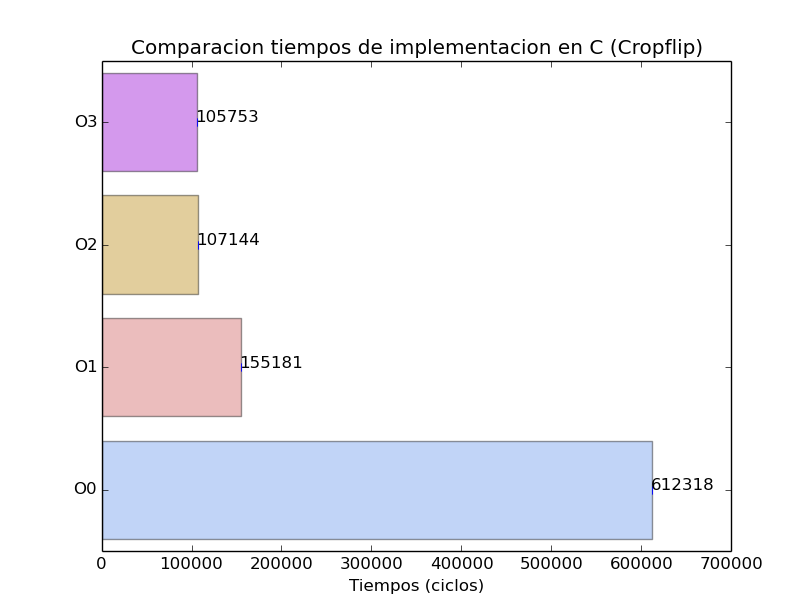
\includegraphics[width=350pt]{cropCompC.png}
En el gr\'{a}fico se nota la clara diferencia entre las corridas con optimizaciones y sin ellas. El criterio fue el mismo que aplicamos en los experimentos de m\'{a}s adelante (Haciendo 1000 iteraciones).

\newpage

\textbf{Experimento 1.3)}\\ \\ 
En este experimento consideraremos diferentes criterios realizando siempre 10 mediciones, con outliers, sin ellos, y agregando programas en C++ que trabajen en simult\'{a}neo.\\ \\

\noindent \textbf{a)} \indent \textbf{Resultados:}\\ \\ 422861, 242136, 186857,\\ 194709, 234097, 221979,\\ 247912, 227976, 223245,\\ 200770.\\ \\ \\

\noindent\textbf{b)} \indent \textbf{Resultados:}\\ \\ 289209, 302654, 258757,\\ 254428, 248527, 254606,\\ 260391, 338981, 373612,\\ 280937 \\ \\ \\

\noindent \textbf{c)} \\ \textbf{10 mediciones}\\Esperanza: 240254.2  Desv\'{i}o standard: 67250.78758  Varianza: 4522668429.51111\\
\noindent \textbf{10 mediciones con el programa en simult\'{a}neo:}\\Esperanza: 286210.2  Desv\'{i}o standard: 41607.01932
Varianza: 1731144056.62222\\ \\ \\
\textbf{d)} \textbf{10 mediciones sin 2 outliers:}\\Esperanza: 224103  Desv\'{i}o standard: 18595.78063  Varianza: 345803057.14286\\ \\ \\

\noindent \textbf{e)} \\ INSERT GRAFICOU HERE \\ \\ \\

Luego de observar estas mediciones hemos notado una varianza demasiado alta (y, en consecuencia, una falta de confiabilidad en las mediciones), por lo tanto, luego de probar con distintos m\'{e}todos de medici\'{o}n decidimos tomar el promedio de 1000 mediciones 10 veces, eliminar outliers y calcular luego nuevamente el promedio de las mediciones restantes.

\newpage

\textbf{Experimento 1.4)}\\ \\

Este experimento comparar\'{a} la performance de las implementaciones C y assembler que aplican el filtro cropflip (siguiendo el modelo de procesamiento secuencial y vectorial, respectivamente), probamos la implementaci\'{o}n en C con 4 distintos flags de optimizaci\'{o}n.

\begin{itemize}

\item \textbf{asm-} 46671 ciclos\\
\item \textbf{C O3-} 106740 ciclos\\
\item \textbf{C O2-} 106859 ciclos\\
\item \textbf{C O1-} 156148 ciclos\\
\item \textbf{C O0-} 613445 ciclos\\ \\ \\

\end{itemize}



NOTA: las l\'{i}neas peque\~nas azules en el tope de las barras representan el desv\'{i}o est\'{a}ndar del promedio de las mediciones que estamos mostrando.

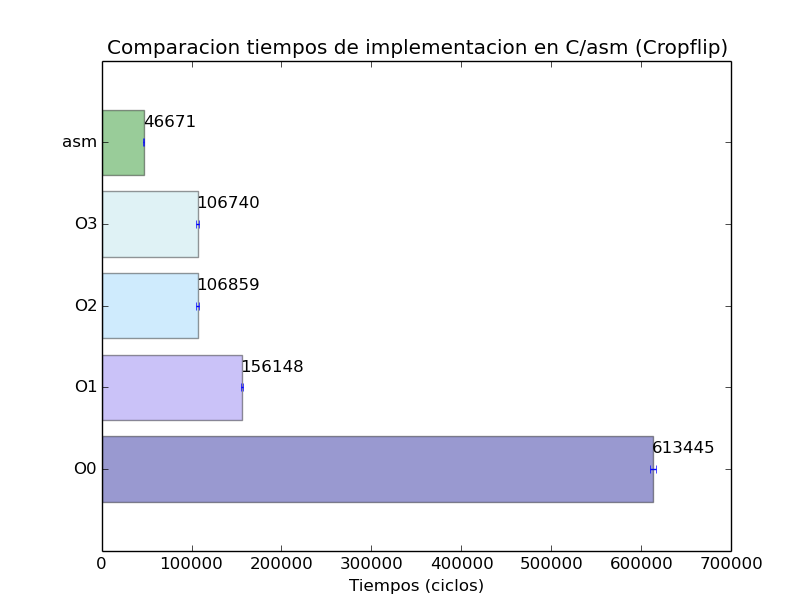
\includegraphics[width=300pt]{CompCasm1.png}

Se observa en este experimento una notoria ventaja (en eficiencia temporal) del procesamiento vectorial de datos sobre el secuencial, incluso luego de haber aplicado las optimizaciones sobre el secuencial (que redujeron mucho el tiempo de procesamiento) la implementaci\'{o}n de assembler pudo aplicar el filtro mucho m\'{a}s r\'{a}pido y de manera m\'{a}s efectiva, mientras que entre las optimizaciones O2-O3 no hubo diferencia casi, indicando que no parece ser posible optimizar mucho m\'{a}s la implementaci\'{o}n en C.\\ \\ \\ \\


\textbf{Experimento 1.5) Cropflip - cpu vs bus de memoria}\\ \\

blablalbla pregrafico

blablabla postgrafico \\ \\ \\ \\

\textbf{Experimento 2.1) Sierpinski - secuencial vs vectorial}\\ \\

Este experimento comparar\'{a} la performance de las implementaciones C y assembler que aplican el filtro sierpinski (siguiendo el modelo de procesamiento secuencial y vectorial, respectivamente), probamos la implementaci\'{o}n en C con 4 distintos flags de optimizaci\'{o}n.

\begin{itemize}


\item \textbf{asm-} 1618682 ciclos\\
\item \textbf{C O3-} 4114385  ciclos\\
\item \textbf{C O2-} 10599598 ciclos\\
\item \textbf{C O1-} 17026398 ciclos\\
\item \textbf{C O0-} 24125694 ciclos\\ \\ \\

\end{itemize}

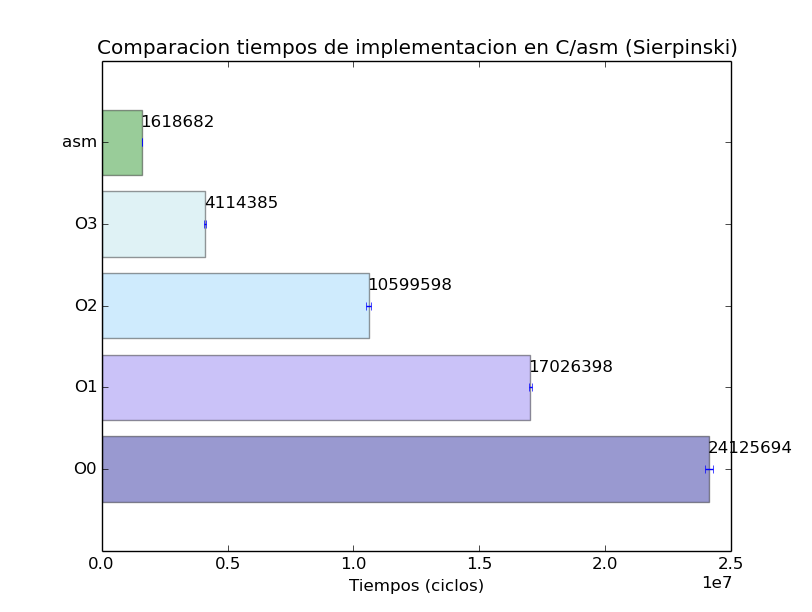
\includegraphics[width=350pt]{CompCasm2.png}

En este experimento la ventaja de usar SIMD sigui\'{o} not\'{a}ndose con fuerza, mostrando una gran diferencia cuando es contrastado su tiempo de ejecuci\'{o}n con el de las distintas optimizaciones de la implementaci\'{o}n en C, si bien en este caso se not\'{o} que la optimizaci\'{o}n O3 tiene un gran impacto comparada con la O2. \\ \\ \\ \\

\textbf{Experimento 2.1) Sierpinski - cpu vs bus de memoria}\\ \\

\newpage

\textbf{Experimento 3.1) Bandas - saltos condicionales}



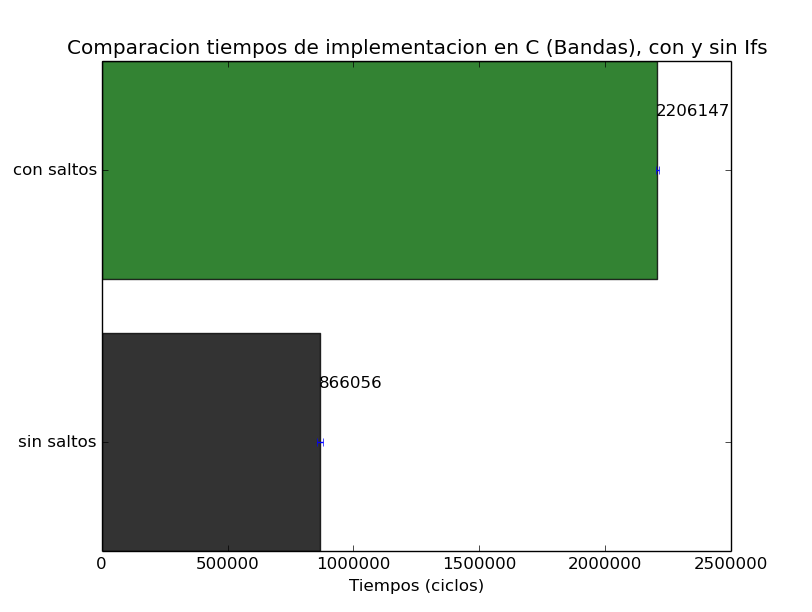
\includegraphics[width=350pt]{cmpIFS.png}

\newpage

\textbf{Experimento 3.2) Bandas - secuencial vs vectorial}\\ \\

Este experimento comparar\'{a} la performance de las implementaciones C y assembler que aplican el filtro bandas (siguiendo el modelo de procesamiento secuencial y vectorial, respectivamente), probamos la implementaci\'{o}n en C con 4 distintos flags de optimizaci\'{o}n.

\begin{itemize}

\item \textbf{asm-}  516916 ciclos\\
\item \textbf{C O3-} 2205562 ciclos\\
\item \textbf{C O2-} 2165530 ciclos\\
\item \textbf{C O1-} 2214220 ciclos\\
\item \textbf{C O0-} 6931576 ciclos\\ \\ \\

\end{itemize}

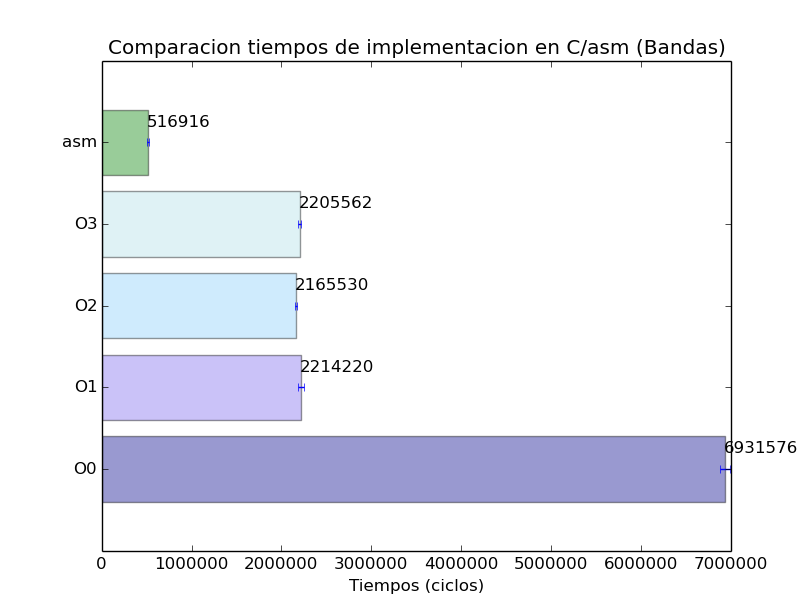
\includegraphics[width=350pt]{CompCasm3.png}

\newpage

\textbf{Experimento 4.1) Motion Blur - secuencial vs vectorial}\\ \\

Este experimento comparar\'{a} la performance de las implementaciones C y assembler que aplican el filtro motion blur (siguiendo el modelo de procesamiento secuencial y vectorial, respectivamente), probamos la implementaci\'{o}n en C con 4 distintos flags de optimizaci\'{o}n.

\begin{itemize}

\item \textbf{asm-}  2030949 ciclos
\item \textbf{C O3-} 4698057 ciclos\\
\item \textbf{C O2-} 4889967 ciclos\\
\item \textbf{C O1-} 5513945 ciclos\\
\item \textbf{C O0-} 17694922 ciclos\\\\ \\ \\

\end{itemize}

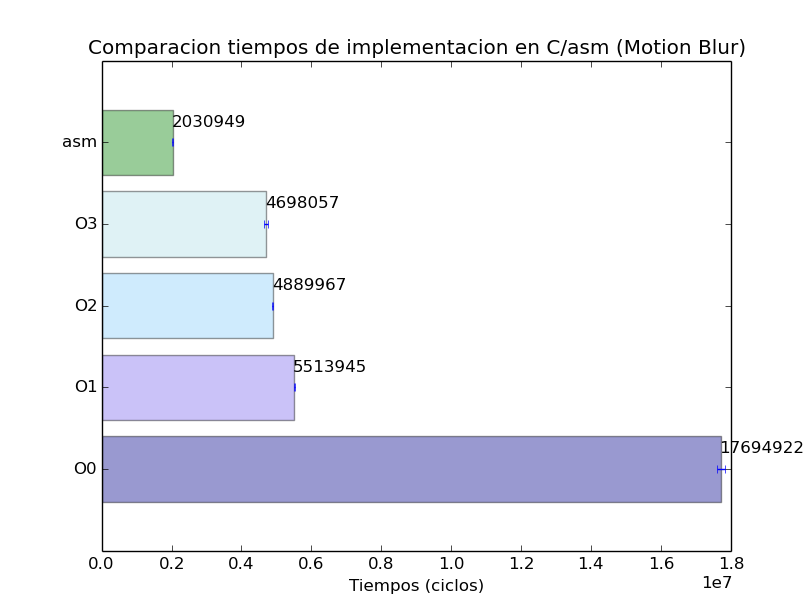
\includegraphics[width=350pt]{CompCasm4.png}

En este experimento, nuevamente, la implementaci\'{o}n de assembler mostr\'{o} una clara diferencia (positiva) con las distintas optimizaciones de la de C, mientras que en C no se pudo optimizar el c\'{o}digo mucho m\'{a}s all\'{a} de la primera optimizaci\'{o}n.

\newpage

\section{Conclusi\'{o}n}



\end{document}
